\PassOptionsToPackage{dvipsnames,table}{xcolor}
\documentclass[11pt,a4paper]{article}

\usepackage{Act}


\begin{document}
\input{\detokenize{/home/fenarius/Travail/Cours/cpge-info/latex/Macros.tex}}
\newcommand{\SPATH}{/home/fenarius/Travail/Cours/cpge-info/docs/mp2i/files/}

\ModeExercice

\lhead{{\sc mpi --} {\bf Préparation aux oraux}}
\rhead{2024}
\setboolean{corrige}{false}
\begin{center}
	\textbf{\Large Sujet F}
\end{center}


\setcounter{Exercise}{0}

\newcommand{\cn}[1]{\TCircle{\tt #1}}
\psset{arrows=->,treesep=1cm,levelsep=1cm}

\begin{Exercise*}[title = type A]\\
	On s'intéresse dans cet exercice à la compression de chaines de caractères représentant des séquences génétiques codées sur l'alphabet {\tt \{A, C, G, T\}} avec l'algorithme de Huffmann.  On rappelle que le principe de cet algorithme est d'attribuer aux caractères les plus fréquents un code plus court.
	\Question{On veut compresser la séquence $S$={\tt ATGTGATGTCCT}, donner le nombre d'occurrences de chaque caractère dans cet séquence.}
	\tcor{ \begin{tabular}{|l|c|c|c|c|}
			\hline
			Caractère            & A & C & G & T \\
			\hline
			Nombre d'occurrences & 2 & 2 & 3 & 5 \\
			\hline
		\end{tabular}}
	\Question{Construire l'arbre de Huffman associé à la compression de $S$.}
	\tcor{
		\begin{center}
			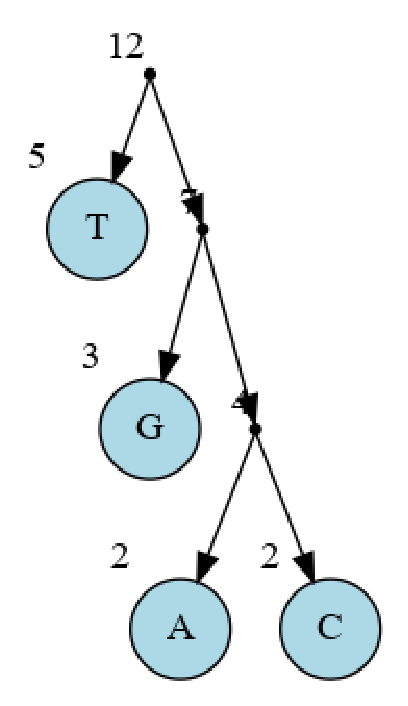
\includegraphics[height=5cm]{hf.eps}
		\end{center}
	}
	\Question{Donner les codes obtenus pour chacun des quatre caractères {\tt A, C, G} et {\tt T}. En déduire le taux de compression de l'algorithme. On supposera qu'initialement la séquence est codée en {\sc ascii} et que donc chacun des caractères occupe un octet et on ne tiendra pas compte de la taille de l'arbre.}
	\tcor{
	\begin{itemize}
		\item Code pour {\tt T} = {\tt 0}
		\item Code pour {\tt G} = {\tt 10}
		\item Code pour {\tt A} = {\tt 110}
		\item Code pour {\tt C} = {\tt 111}
	\end{itemize}

	\Ret
	Comme indiqué sur l'arbre {\tt T} apparaît 5 fois, {\tt G} 3 fois et {\tt A} et {\tt C} chacun deux fois. La taille finale du code est donc : $5 \times 1 + 3\times 2 + 2\times 3 + 2 \times 3 = 23$ bits, alors le code initial contenait $12$ caractères codés sur 8 bits chacun donc $96$ octets, le taux de compression est donc de $\dfrac{23}{96} \simeq 24 \%$.
	}
	\Question{Quelle structure de données abstraite est utilisée pour implémenter cet algorithme ? Quelle en est l'implémentation usuelle ?}
	\tcor{On doit disposer d'une file de priorité afin d'y stocker les sous arbres avec le total du nombre d'occurrences qu'il contiennent. Une file de priorité est usuellement implémentée en utilisant un tas binaire min. Les opérations d'extraction et d'insertion d'un élément sont alors en complexité logarithmique de la taille du tas.}
	\Question{Proposer un type en OCaml permettant de représenter un arbre de Huffmann.}
	\ifcorrige
		\corpartOCaml{huff.ml}{}{}{1}{3}
	\fi
\end{Exercise*}

\begin{Exercise*}[title = {type B}]\\
	On dispose d'un \textit{système monétaire} c'est-à-dire d'un ensemble de valeurs possibles pour les pièces et les billets. Le problème du rendu de monnaie consiste à déterminer le nombre minimal de pièces à utiliser pour former une somme donnée. On supposera que les valeurs des pièces et des billets sont des entiers de même que la somme à rendre et que le système monétaire contient toujours la valeur 1 (de cette façon, le problème admet toujours une solution). Les fonctions demandées dans cet exercice sont à écrire en OCaml et on donnera le système monétaire sous la forme de la liste \textit{triée dans l'ordre décroissant} des valeurs des pièces. Par exemple, la liste \mintinline{ocaml}{[500; 200; 100; 50; 20; 10; 5; 2; 1]} est un système monétaire correct et le nombre minimal de pièces pour rendre la somme {\tt 17} est {\tt 3} (obtenue en utilisant {\tt 10 + 5 + 2}.). D'autre part, on s'interdit dans cet exercice l'utilisation des aspects impératifs du langage OCaml (en particulier les boucles et les références.)

    \Question{Ecrire une fonction {\tt verifie : int list -> bool} qui prend en argument un systeme monétaire et renvoie un booléen indiquant si ce système est valide (c'est à dire la liste des valeurs est rangée dans l'ordre décroissant et se termine par 1).}
    \ifcorrige
    \corpartOCaml{rm.ml}{}{}{1}{5}
    \fi
    \Question{On considère dans un premier temps la méthode consistant à rendre toujours la pièce de plus forte valeur possible. A quelle famille d'algorithme appartient cette méthode ? Justifier.}
    \tcor{Il s'agit d'un algorithme glouton car on effectue un choix local optimal (dans le sens où la somme à rendre diminue le plus possible) à chaque étape.}
    \Question{En utilisant un exemple de votre choix, montrer que cette méthode ne fournit pas toujours le nombre minimal de pièces.}
    \tcor{On peut par exemple considérer le système monétaire \mintinline{ocaml}{[5; 4; 3; 1]} et former la somme 7, l'algorithme glouton utilise alors 3 pièces (5+1+1) alors qu'on peut n'en utiliser que  2 (4+3).}
    \Question{Donner une implémentation de cette méthode sous la forme d'une fonction {\tt monnaie : int list -> int -> int} prenant en argument un système monétaire ainsi qu'une somme et renvoyant le nombre de pièces.}
    \ifcorrige
    \corpartOCaml{rm.ml}{}{}{7}{11}
    \fi
    \Question{On veut maintenant résoudre ce problème par programmation dynamique.
        On note $(p_i)_{0 \leqslant i \leqslant n}$ les valeurs des pièces rangées dans l'ordre décroissant, et on note $m(S,k)$ le nombre minimal de pièces pour rendre la somme $S$ en utilisant seulement les pièces $p_k, \dots, p_{n-1}$. On convient que $m(S, k) = +\infty$ si $S \neq0$ et $k \geqslant n$ car on cherche alors à rendre une somme non nulle sans utiliser de pièces. Donner la relation liant $m(S, k)$ à $m(S, k+1)$ si on choisit de ne pas utiliser la pièce $p_k$. De même trouver une relation entre différentes instances du problème lorsqu'on choisit d'utiliser $p_k$ (dans ce cas, on a nécessairement $S \geqslant p_k$).
    }
    \tcor{
    \begin{itemize}
    \item si $S<p_k$ alors $m(S, k) = m(S, k+1)$
    \item sinon, $m(S,k)    = \min\left\{ 1 + m(S-p_k,k), m(S,k+1) \text{  }\right\}$
    \end{itemize}    
    D'autre part, $m(S, 0) = 0$.
    }
    \Question{Ecrire une fonction {\tt dynamique : int list -> int -> int} qui résoud le problème par programmation dynamique, on pourra utiliser la valeur {\tt Int.max} de OCaml afin d'indiquer que la résolution est impossible (nombre infini de pièces).}
    \ifcorrige
    \corpartOCaml{rm.ml}{}{}{13}{20}
    \fi

\end{Exercise*}


\end{document}